% Unofficial NYIT Poster Template
% a fork of https://github.com/anishathalye/gemini
% also refer to https://github.com/k4rtik/uchicago-poster

\documentclass[final]{beamer}

% ====================
% Packages
% ====================

\usepackage[T1]{fontenc}
\usepackage{lmodern}
% \usepackage[size=custom,width=120,height=72,scale=1.0]{beamerposter}
\usepackage[size=custom,width=91.44,height=60.96,scale=1.0]{beamerposter}
\usetheme{gemini}
\usecolortheme{nyit}
\usepackage{graphicx}
\usepackage{calc}
\usepackage{booktabs}
\usepackage{doi}
\usepackage[numbers]{natbib}
\usepackage[patch=none]{microtype}
\usepackage{tikz}
\usetikzlibrary{positioning, shapes, calc, arrows}
\usepackage{pgfplots}
\pgfplotsset{compat=1.18}
\usepackage{anyfontsize}
\usepackage{minted}
\setminted{
	style = lovelace,
	% frame = lines,
	tabsize = 4,
	breaklines,
	% linenos
}

\usepackage{hyperref}
\hypersetup{
	colorlinks = true,
	urlcolor = catalina-blue
}

\pdfstringdefDisableCommands{%
\def\translate#1{#1}%
}

% ====================
% Lengths
% ====================

% If you have N columns, choose \sepwidth and \colwidth such that
% (N+1)*\sepwidth + N*\colwidth = \paperwidth
\newlength{\sepwidth}
\newlength{\colwidth}
\setlength{\sepwidth}{0.025\paperwidth}
\setlength{\colwidth}{0.3\paperwidth}

\newcommand{\separatorcolumn}{\begin{column}{\sepwidth}\end{column}}

% ====================
% Title
% ====================

\title{Visualization and Connectedness of %\\
Quadratic Julia Sets}

\author{Emily Prieto}

% \institute[shortinst]{\inst{1} Some Institute \samelineand \inst{2} Another Institute}

% ====================
% Footer (optional)
% ====================

\footercontent{
	% \href{https://www.example.com}{https://www.example.com} \hfill
	New York Tech Math Day 2025 \hfill
	\href{mailto:eprieto@nyit.edu}{\color{white} eprieto@nyit.edu}}
% (can be left out to remove footer)

% ====================
% Logo (optional)
% ====================

% use this to include logos on the left and/or right side of the header:
% \logoright{\includegraphics[height=7cm]{logo1.pdf}}
% \logoleft{\includegraphics[height=7cm]{logo2.pdf}}

\usepackage{amsmath}
\usepackage{amssymb}
\usepackage{amsfonts}
\usepackage{amsthm}

\newcommand{\setbold}{\mathbf}
\newcommand{\CC}{\setbold{C}}
\newcommand{\RR}{\setbold{R}}
\newcommand{\NN}{\setbold{N}}

% \newtheorem*{theorem}{Theorem}
% \newtheorem*{lemma}{Lemma}
\newcommand{\taggedqed}{\rlap{$\quad \Box$}}
\newcommand{\noqed}{\renewcommand{\qedsymbol}{}}

% ====================
% Body
% ====================

\begin{document}
% \addtobeamertemplate{headline}{}
% {
%     \begin{tikzpicture}[remember picture,overlay]
%       \node [anchor=north west, inner sep=3cm] at ([xshift=0.0cm,yshift=1.0cm]current page.north west)
%       {
\includegraphics[height=5.0cm]{logos/uc-logo-white.eps}}; % also try shield-white.eps
%       \node [anchor=north east, inner sep=3cm] at ([xshift=0.0cm,yshift=2.5cm]current page.north east)
%       {
\includegraphics[height=8.0cm]{logos/cs-logo-white.png}};
%     \end{tikzpicture}
% }

\begin{frame}[t]
\begin{columns}[t]
\separatorcolumn

\begin{column}{\colwidth}

	\begin{block}{What is a Julia set?}

		The \textbf{Julia set} of a function $f$ is a
		region in the complex plane that has certain
		properties as we repeatedly apply $f$.
		Julia sets are known for forming intricate
		patterns and having a fractal-like appearance.

		This project studies the Julia sets of
		\textbf{quadratic maps} of the form
		$Q_c(z) = z^2 + c$ where $c$ is a complex number.
		We define the following notation for repeated function application: \[
			Q_c^{m}(z) = (\overbrace{\vphantom{(}Q_c \circ \cdots \circ Q_c}^{m\ \text{times}})(z)
		\]

		Formally, the \textbf{filled Julia set} $K(Q_c)$
		is the subset of the complex plane that remains bounded
		under repeated application of $Q_c$. \[
			% FIXME: different arrowheads
			K(Q_c) := \left\{ z \in \CC : |Q_c^{m}(z)| \nrightarrow \infty\ \text{as}\ m \rightarrow \infty \right\}
		\]
		The \textbf{Julia set} $J(Q_c) := \partial{} K(Q_c)$ is the boundary
		of the filled Julia set.

	\end{block}

	\begin{alertblock}{Escape Criteria}
		We can prove the following property, which will
		be very useful in rendering filled Julia sets.

    \textit{Lemma.}
		If $|Q_c^{m}(z)| > k$
		for some $m$, then $|Q_c^{n}(z)| \rightarrow \infty$ as $n \rightarrow \infty$,
    where $k = \max(|c|, 2)$.

		\textit{Proof.}
		Let $w = Q_c^{m}(z)$. Then $Q_c^{n}(z) = Q_z^{m + \ell}(z) = Q_c^{\ell}(Q_c^{m}(z))$.
		$|w| > k$, so $|w| > |c|$ and $|w| > 2$. Thus $|w| - 1 > 1$.
		By the \textbf{inverse triangle inequality} ($|a + b| \ge |a| - |b|$),
		\begin{align*}
			|Q_c(w)| = |w^2 + c| &\ge |w^2| - |c| \\
								 &> |w^2| - |w| \\
								 &= (|w| - 1)|w| > |w| > k
		\end{align*}
		Since $Q_c^{\ell}(w) = Q_c(Q_c^{\ell - 1}(w))$, we have \[
			|Q_c^{\ell}(w)| > |Q_c^{\ell - 1}(w)| > \cdots > |Q_c^{2}(w)| >|Q_c^{1}(w)| > |w| > k
		\]
		So when $|Q_c^{m}(z)| > k$, the sequence \[
			\left\{ |Q_c^{m + 1}(z)|, |Q_c^{m + 2}(z)|, \ldots \right\}
		\] is strictly increasing, so its limit goes to infinity. \hfill $\square$

		We use this lemma in the code to determine whether a particular
		seed $z$ should be part of $K(Q_c)$.
	\end{alertblock}

\end{column}

\separatorcolumn

\begin{column}{\colwidth}

	\begin{block}{Python Implementation}
		We use NumPy to perform the computations and Matplotlib
		to visualize the final result.
		We first select a rectangular subset of the complex plane
		and a resolution. We will check if every point on the lattice
		\inputminted[firstline=102,lastline=103]{python}{../visualize.py}
		remains bounded.
		We do this by applying $Q_c$ a set number of times to each seed value.
		If $Q^{m}_c(z)$ does not exceed our escape criteria after a large number
    of iterations, we consider it part of $K(Q_c)$.
		We use a NumPy matrix to concisely express these operations:
		\inputminted[firstline=108,lastline=113]{python}{../visualize.py}
		This produces another matrix, which we scale to the interval
		$[0, 1]$ and render using Matplotlib:
		\inputminted[firstline=118,lastline=118]{python}{../visualize.py}
		To produce a better image, we color the plane
		by how quickly each point exceeds the escape criteria.
		More iterations and a higher resolution
		will result in more accurate images, but will be more expensive to compute.
	\end{block}

	\begin{block}{GPU Shader Implementation}
		The algorithm here is identical to that used in the Python
		implementation.
		It is much faster by virtue of running in parallel for each seed
		on the lattice.
		It is available on Shadertoy here: \href{https://www.shadertoy.com/view/tXfXWj}{shadertoy.com/view/tXfXWj}.
		\inputminted[firstline=271,lastline=278]{glsl}{../render.glsl}
	\end{block}
\end{column}

\separatorcolumn

\begin{column}{\colwidth}
	\begin{block}{Conclusions}
		% \begin{figure}
		%   \centering
		%   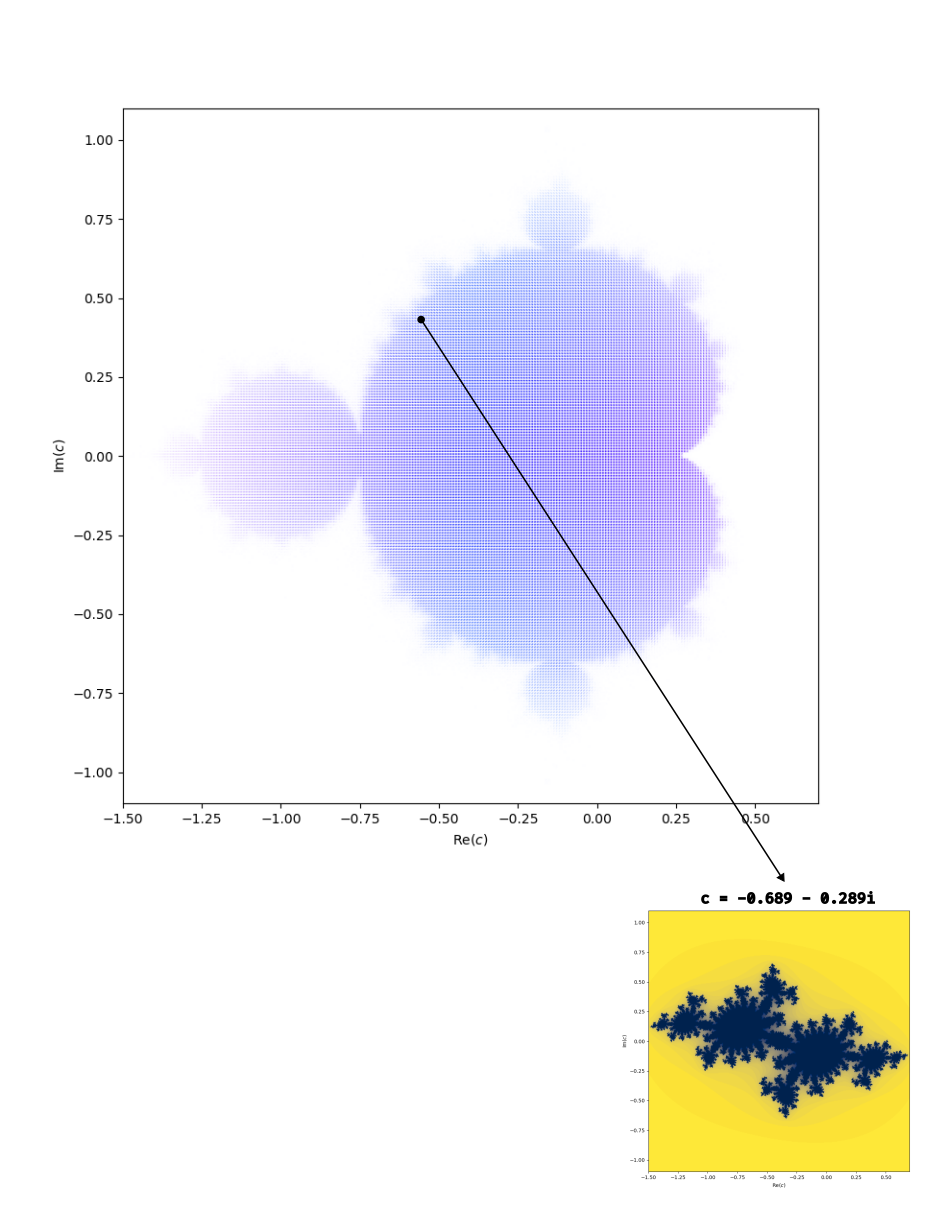
\includegraphics[width=8in]{../figures/connectedness.png}
		%   \caption{....}
		% \end{figure}

		Through diverse visualization methods, various facts about
		quadratic Juila sets present themselves.

		\heading{Origin Symmetry}
		All quadratic Julia sets are symmetric about the origin.
		This is a consequence of the definition of $Q_c$. \[
			Q_c(z) = z^2 + c = (-z)^2 + c = Q_c(-z)
		\]

		\heading{Other Symmetry: $\alpha + \beta i \in K(Q_c) \iff -\alpha + \beta i \in K(Q_{\overline{c}})$}
		When we reflect $c$ over the real axis, $K(Q_c)$
		is reflected over the imaginary axis.
		See Figure \ref{fig:mandelbrot} for an example.
		\begin{gather*}
			Q_{\gamma + \delta i}(\alpha + \beta i) = (\alpha + \beta i)^2 + (\gamma + \delta i) = (\alpha^2 - \beta^2 + \gamma) + (2\alpha \beta + \delta)i \\
			Q_{\gamma - \delta i}(-\alpha + \beta i) = (-\alpha + \beta i)^2 + (\gamma - \delta i) = (\alpha^2 - \beta^2 + \gamma) - (2\alpha \beta + \delta)i
			% Q_{\gamma - \delta i}(\alpha + \beta i) = (\alpha + \beta i)^2 + (\gamma - \delta i) = (\alpha^2 - \beta^2 + \gamma) + (2\alpha \beta - \delta)i \\
			% Q_{\gamma + \delta i}(-\alpha + \beta i) = (-\alpha + \beta i)^2 + (\gamma - \delta i) = (\alpha^2 - \beta^2 + \gamma) - (2\alpha \beta + \delta)i
		\end{gather*}

		\heading{Connectedness of $K(Q_c)$}
		When $c$ is near the origin, $K(Q_c)$
		is \textbf{2-connected}.
		When $c$ is on the boundary of the Mandelbrot set,
		$K(Q_c)$ is observed as \textbf{1-connected}.
		When $c$ is outside the Mandelbrot set,
		$K(Q_c)$ is \textbf{disconnected}.

		We arrived at this result by rendering the image in Figure \ref{fig:mandelbrot},
		which is a mosaic of filled Julia sets.
		Each of the $2^{16}$ subimages represents $K(Q_c)$,
		and is centered on $c$ on the complex plane.
		When $K(Q_c)$ is disconnected, it is not visible in the mosaic,
		meaning that the shaded region represents precisely those $Q_c$
		for which $K(Q_c)$ is connected.

		The 1-connectedness of $K(Q_c)$ at the boundary
		is yet to be analyzed.
		\begin{figure}
			\label{fig:mandelbrot}
			\begin{center}
				\begin{tikzpicture}[x=1.7735in, y=1.6903in, every node/.style={inner sep=0in, outer sep=0in}]
					\node (mandelbrot) at (-0.4, 0) {
						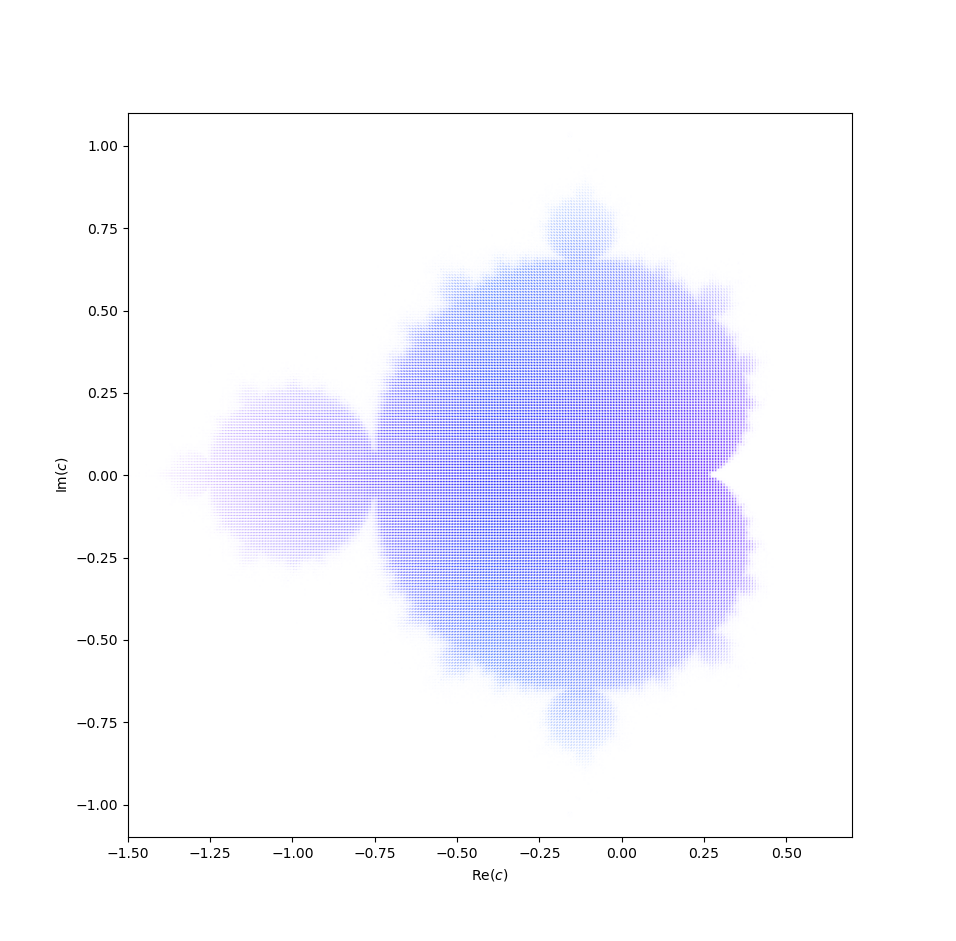
\includegraphics[width=5in]{../figures/dithered-mandelbrot-inverted-ticks.png}
					};

					\node[matrix, right=-5mm of mandelbrot] {
						\node (left-rabbit) {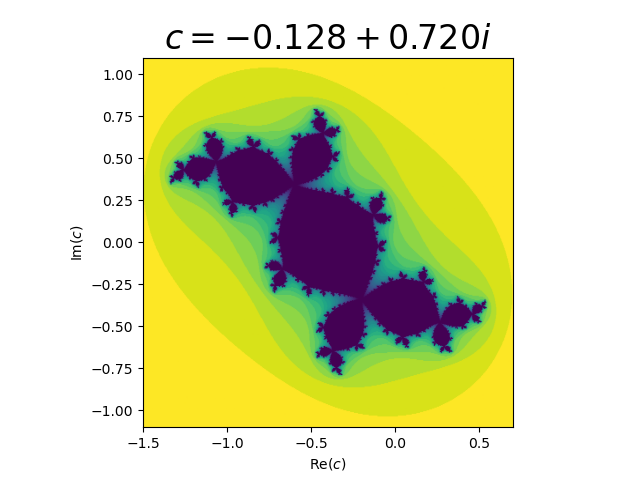
\includegraphics[width=2.5in]{../figures/left-rabbit-ticks.png}}; \\
						\node (right-rabbit) {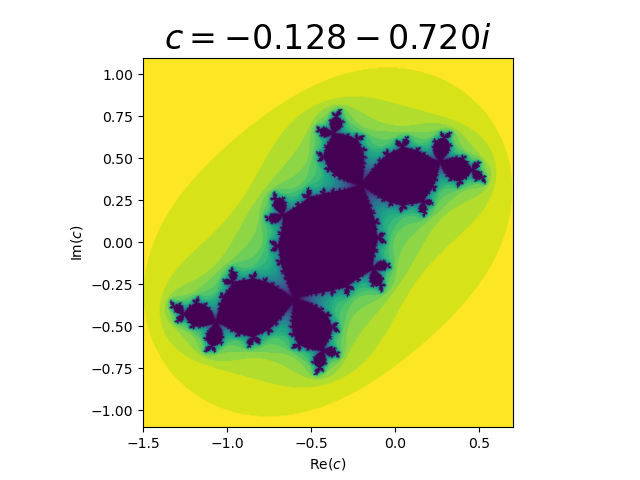
\includegraphics[width=2.5in]{../figures/right-rabbit-ticks.png}}; \\
					};

					\node[matrix, left=-5mm of mandelbrot] {
						\node (exterior) {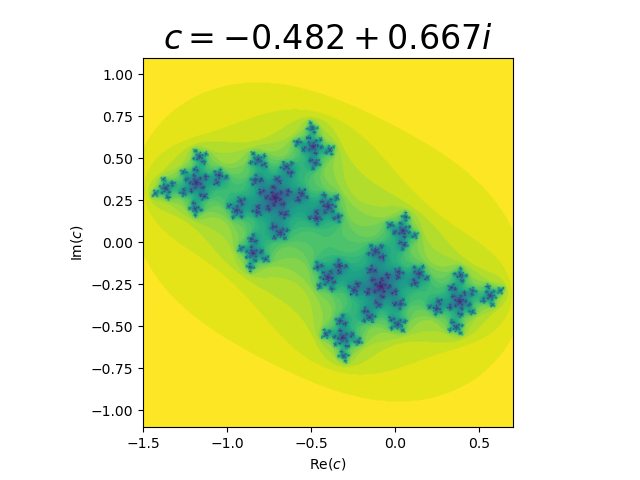
\includegraphics[width=2.5in]{../figures/exterior-ticks.png}}; \\
						\node (boundary) {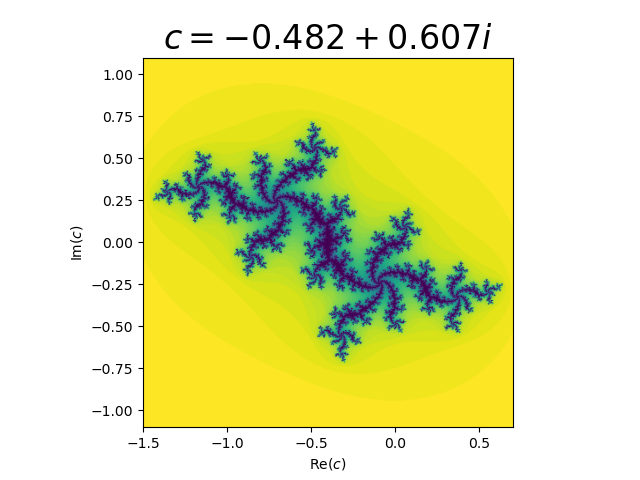
\includegraphics[width=2.5in]{../figures/boundary-ticks.png}}; \\
						\node (interior) {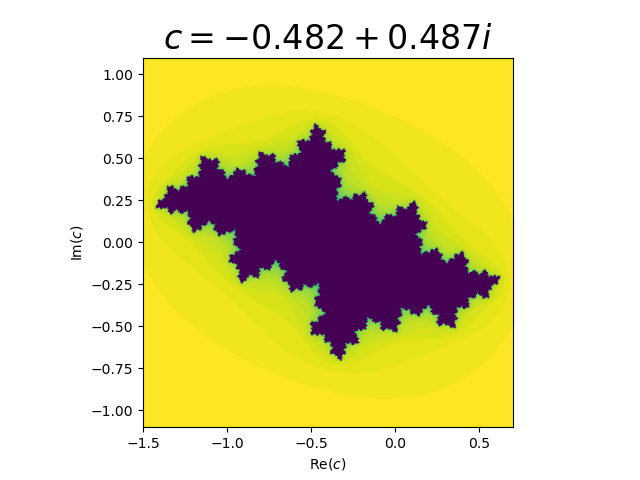
\includegraphics[width=2.5in]{../figures/interior-ticks.png}}; \\
					};

					\coordinate (left-rabbit-c) at (-0.128, 0.720);
					\coordinate (right-rabbit-c) at (-0.128, -0.720);
					\coordinate (exterior-c) at (-0.482, 0.667);
					\coordinate (boundary-c) at (-0.482, 0.607);
					\coordinate (interior-c) at (-0.482, 0.487);

					% \filldraw (0, 0) circle (1pt);
					\foreach \c in {left-rabbit,right-rabbit,exterior,boundary,interior} {
						\filldraw (\c-c) circle (1pt);
					}

					\draw[dotted] (interior-c) -- (boundary-c) -- (exterior-c);
					\draw[dotted] (-1.46, -0.012) -- (0.7, -0.012);
					\path[-latex]
						(exterior-c) edge ($(exterior.east) - (0.28in, 0)$)
						(boundary-c) edge ($(boundary.east) - (0.28in, 0)$)
						(interior-c) edge ($(interior.east) - (0.27in, 0)$)
						(left-rabbit-c) edge ($(left-rabbit.west) + (0.24in, 0)$)
						(right-rabbit-c) edge ($(right-rabbit.west) + (0.24in, 0)$);
				\end{tikzpicture}
				%\begin{minipage}{2.5in}
				%	\begin{tabular}{c}
				%		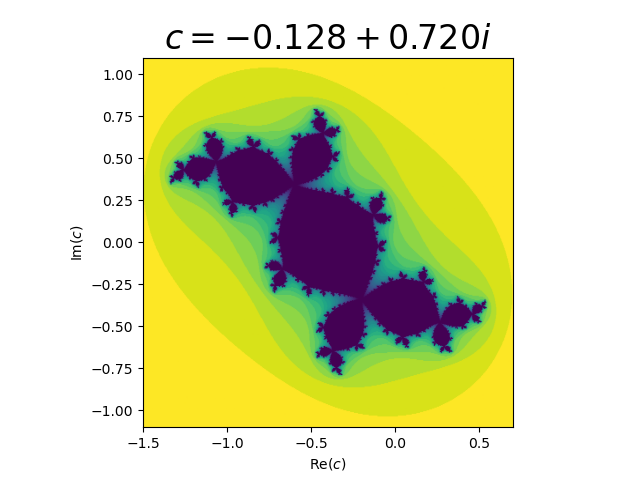
\includegraphics[width=2.5in]{../figures/left-rabbit-ticks.png} \\
				%		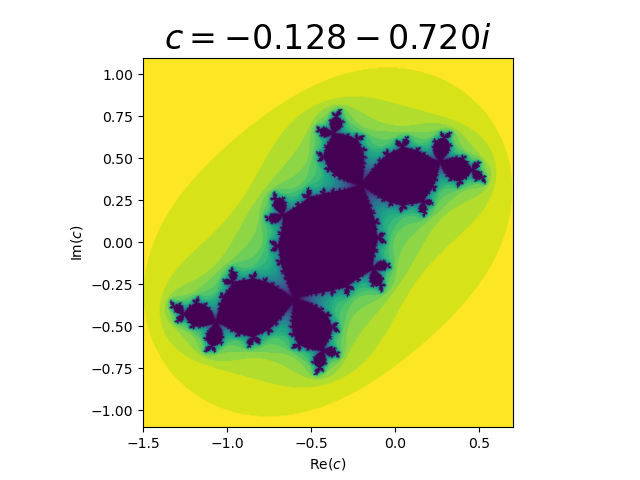
\includegraphics[width=2.5in]{../figures/right-rabbit-ticks.png}
				%	\end{tabular}
				%\end{minipage}
				%\begin{minipage}{5in}
				%	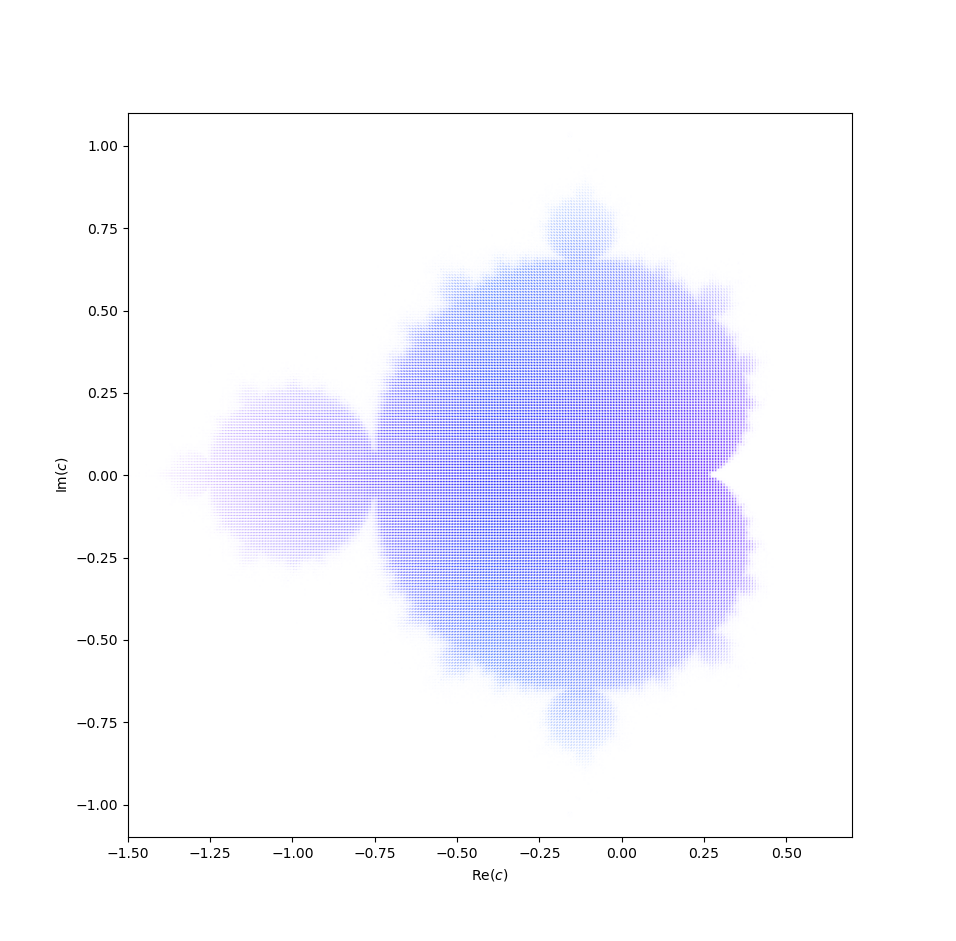
\includegraphics[width=5in]{../figures/dithered-mandelbrot-inverted-ticks.png}
				%\end{minipage}
				%\begin{minipage}{2.5in}
				%	\begin{tabular}{c}
				%		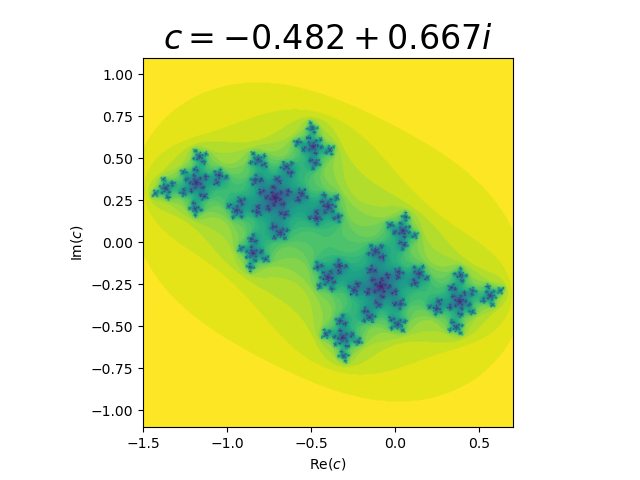
\includegraphics[width=2.5in]{../figures/exterior-ticks.png} \\
				%		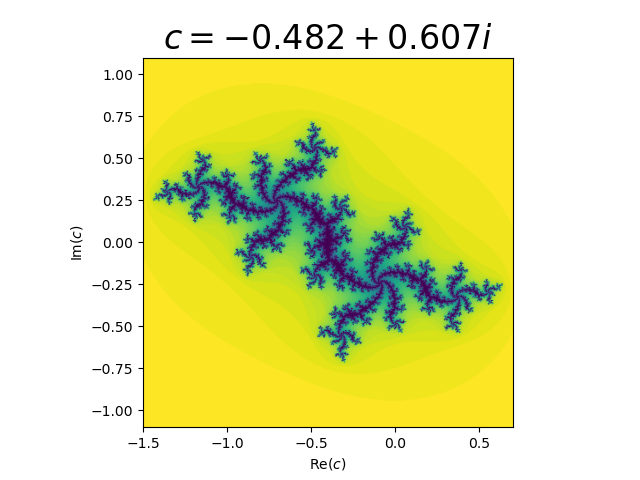
\includegraphics[width=2.5in]{../figures/boundary-ticks.png} \\
				%		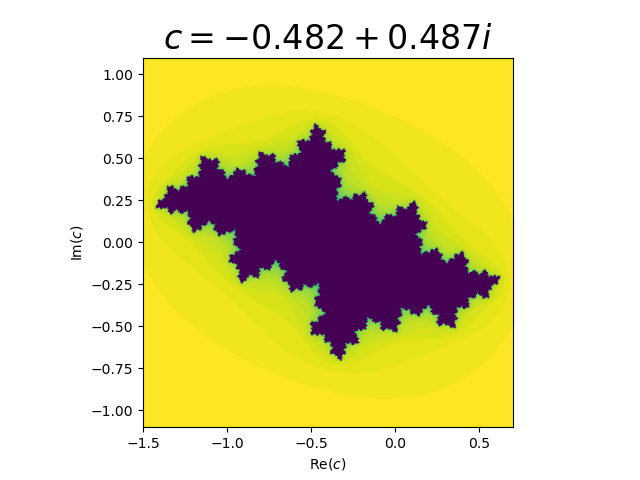
\includegraphics[width=2.5in]{../figures/interior-ticks.png}
				%	\end{tabular}
				%\end{minipage}
			\end{center}
			\caption{Selected subimages of the Mandelbrot mosaic.}
		\end{figure}
	\end{block}


	% \begin{block}{References}

	% 	\nocite{*}
	% 	\footnotesize{\bibliographystyle{plainnat}\bibliography{poster}}

	% \end{block}

\end{column}

\separatorcolumn
\end{columns}
\end{frame}

\end{document}
